% Options for packages loaded elsewhere
\PassOptionsToPackage{unicode}{hyperref}
\PassOptionsToPackage{hyphens}{url}
%
\documentclass[
  ignorenonframetext,
]{beamer}
\usepackage{pgfpages}
\setbeamertemplate{caption}[numbered]
\setbeamertemplate{caption label separator}{: }
\setbeamercolor{caption name}{fg=normal text.fg}
\beamertemplatenavigationsymbolsempty
% Prevent slide breaks in the middle of a paragraph
\widowpenalties 1 10000
\raggedbottom
\setbeamertemplate{part page}{
  \centering
  \begin{beamercolorbox}[sep=16pt,center]{part title}
    \usebeamerfont{part title}\insertpart\par
  \end{beamercolorbox}
}
\setbeamertemplate{section page}{
  \centering
  \begin{beamercolorbox}[sep=12pt,center]{part title}
    \usebeamerfont{section title}\insertsection\par
  \end{beamercolorbox}
}
\setbeamertemplate{subsection page}{
  \centering
  \begin{beamercolorbox}[sep=8pt,center]{part title}
    \usebeamerfont{subsection title}\insertsubsection\par
  \end{beamercolorbox}
}
\AtBeginPart{
  \frame{\partpage}
}
\AtBeginSection{
  \ifbibliography
  \else
    \frame{\sectionpage}
  \fi
}
\AtBeginSubsection{
  \frame{\subsectionpage}
}
\usepackage{amsmath,amssymb}
\usepackage{lmodern}
\usepackage{iftex}
\ifPDFTeX
  \usepackage[T1]{fontenc}
  \usepackage[utf8]{inputenc}
  \usepackage{textcomp} % provide euro and other symbols
\else % if luatex or xetex
  \usepackage{unicode-math}
  \defaultfontfeatures{Scale=MatchLowercase}
  \defaultfontfeatures[\rmfamily]{Ligatures=TeX,Scale=1}
\fi
\usetheme[]{Ilmenau}
% Use upquote if available, for straight quotes in verbatim environments
\IfFileExists{upquote.sty}{\usepackage{upquote}}{}
\IfFileExists{microtype.sty}{% use microtype if available
  \usepackage[]{microtype}
  \UseMicrotypeSet[protrusion]{basicmath} % disable protrusion for tt fonts
}{}
\makeatletter
\@ifundefined{KOMAClassName}{% if non-KOMA class
  \IfFileExists{parskip.sty}{%
    \usepackage{parskip}
  }{% else
    \setlength{\parindent}{0pt}
    \setlength{\parskip}{6pt plus 2pt minus 1pt}}
}{% if KOMA class
  \KOMAoptions{parskip=half}}
\makeatother
\usepackage{xcolor}
\newif\ifbibliography
\usepackage{color}
\usepackage{fancyvrb}
\newcommand{\VerbBar}{|}
\newcommand{\VERB}{\Verb[commandchars=\\\{\}]}
\DefineVerbatimEnvironment{Highlighting}{Verbatim}{commandchars=\\\{\}}
% Add ',fontsize=\small' for more characters per line
\usepackage{framed}
\definecolor{shadecolor}{RGB}{248,248,248}
\newenvironment{Shaded}{\begin{snugshade}}{\end{snugshade}}
\newcommand{\AlertTok}[1]{\textcolor[rgb]{0.94,0.16,0.16}{#1}}
\newcommand{\AnnotationTok}[1]{\textcolor[rgb]{0.56,0.35,0.01}{\textbf{\textit{#1}}}}
\newcommand{\AttributeTok}[1]{\textcolor[rgb]{0.77,0.63,0.00}{#1}}
\newcommand{\BaseNTok}[1]{\textcolor[rgb]{0.00,0.00,0.81}{#1}}
\newcommand{\BuiltInTok}[1]{#1}
\newcommand{\CharTok}[1]{\textcolor[rgb]{0.31,0.60,0.02}{#1}}
\newcommand{\CommentTok}[1]{\textcolor[rgb]{0.56,0.35,0.01}{\textit{#1}}}
\newcommand{\CommentVarTok}[1]{\textcolor[rgb]{0.56,0.35,0.01}{\textbf{\textit{#1}}}}
\newcommand{\ConstantTok}[1]{\textcolor[rgb]{0.00,0.00,0.00}{#1}}
\newcommand{\ControlFlowTok}[1]{\textcolor[rgb]{0.13,0.29,0.53}{\textbf{#1}}}
\newcommand{\DataTypeTok}[1]{\textcolor[rgb]{0.13,0.29,0.53}{#1}}
\newcommand{\DecValTok}[1]{\textcolor[rgb]{0.00,0.00,0.81}{#1}}
\newcommand{\DocumentationTok}[1]{\textcolor[rgb]{0.56,0.35,0.01}{\textbf{\textit{#1}}}}
\newcommand{\ErrorTok}[1]{\textcolor[rgb]{0.64,0.00,0.00}{\textbf{#1}}}
\newcommand{\ExtensionTok}[1]{#1}
\newcommand{\FloatTok}[1]{\textcolor[rgb]{0.00,0.00,0.81}{#1}}
\newcommand{\FunctionTok}[1]{\textcolor[rgb]{0.00,0.00,0.00}{#1}}
\newcommand{\ImportTok}[1]{#1}
\newcommand{\InformationTok}[1]{\textcolor[rgb]{0.56,0.35,0.01}{\textbf{\textit{#1}}}}
\newcommand{\KeywordTok}[1]{\textcolor[rgb]{0.13,0.29,0.53}{\textbf{#1}}}
\newcommand{\NormalTok}[1]{#1}
\newcommand{\OperatorTok}[1]{\textcolor[rgb]{0.81,0.36,0.00}{\textbf{#1}}}
\newcommand{\OtherTok}[1]{\textcolor[rgb]{0.56,0.35,0.01}{#1}}
\newcommand{\PreprocessorTok}[1]{\textcolor[rgb]{0.56,0.35,0.01}{\textit{#1}}}
\newcommand{\RegionMarkerTok}[1]{#1}
\newcommand{\SpecialCharTok}[1]{\textcolor[rgb]{0.00,0.00,0.00}{#1}}
\newcommand{\SpecialStringTok}[1]{\textcolor[rgb]{0.31,0.60,0.02}{#1}}
\newcommand{\StringTok}[1]{\textcolor[rgb]{0.31,0.60,0.02}{#1}}
\newcommand{\VariableTok}[1]{\textcolor[rgb]{0.00,0.00,0.00}{#1}}
\newcommand{\VerbatimStringTok}[1]{\textcolor[rgb]{0.31,0.60,0.02}{#1}}
\newcommand{\WarningTok}[1]{\textcolor[rgb]{0.56,0.35,0.01}{\textbf{\textit{#1}}}}
\setlength{\emergencystretch}{3em} % prevent overfull lines
\providecommand{\tightlist}{%
  \setlength{\itemsep}{0pt}\setlength{\parskip}{0pt}}
\setcounter{secnumdepth}{-\maxdimen} % remove section numbering
\setbeamertemplate{navigation symbols}{}
\setbeamertemplate{footline}[page number]
\usepackage{amsmath}
\ifLuaTeX
  \usepackage{selnolig}  % disable illegal ligatures
\fi
\IfFileExists{bookmark.sty}{\usepackage{bookmark}}{\usepackage{hyperref}}
\IfFileExists{xurl.sty}{\usepackage{xurl}}{} % add URL line breaks if available
\urlstyle{same} % disable monospaced font for URLs
\hypersetup{
  pdftitle={Multivariate Analysis Lecture 14: More on Classification},
  hidelinks,
  pdfcreator={LaTeX via pandoc}}

\title{Multivariate Analysis Lecture 14: More on Classification}
\author{Zhaoxia Yu\\
Professor, Department of Statistics}
\date{2023-05-18}

\begin{document}
\frame{\titlepage}

\hypertarget{outline}{%
\section{Outline}\label{outline}}

\begin{frame}{Outline}
\begin{itemize}
\tightlist
\item
  Review of LDA
\item
  QDA
\item
  Decision theory

  \begin{itemize}
  \tightlist
  \item
    Equal costs
  \item
    Unequal costs
  \end{itemize}
\end{itemize}
\end{frame}

\hypertarget{review-of-lda}{%
\section{Review of LDA}\label{review-of-lda}}

\begin{frame}[fragile]{Linear Discrminant Analysis}
\protect\hypertarget{linear-discrminant-analysis}{}
\begin{Shaded}
\begin{Highlighting}[]
\NormalTok{knitr}\SpecialCharTok{::}\FunctionTok{include\_graphics}\NormalTok{(}\StringTok{"img/FLDA.png"}\NormalTok{)}
\end{Highlighting}
\end{Shaded}

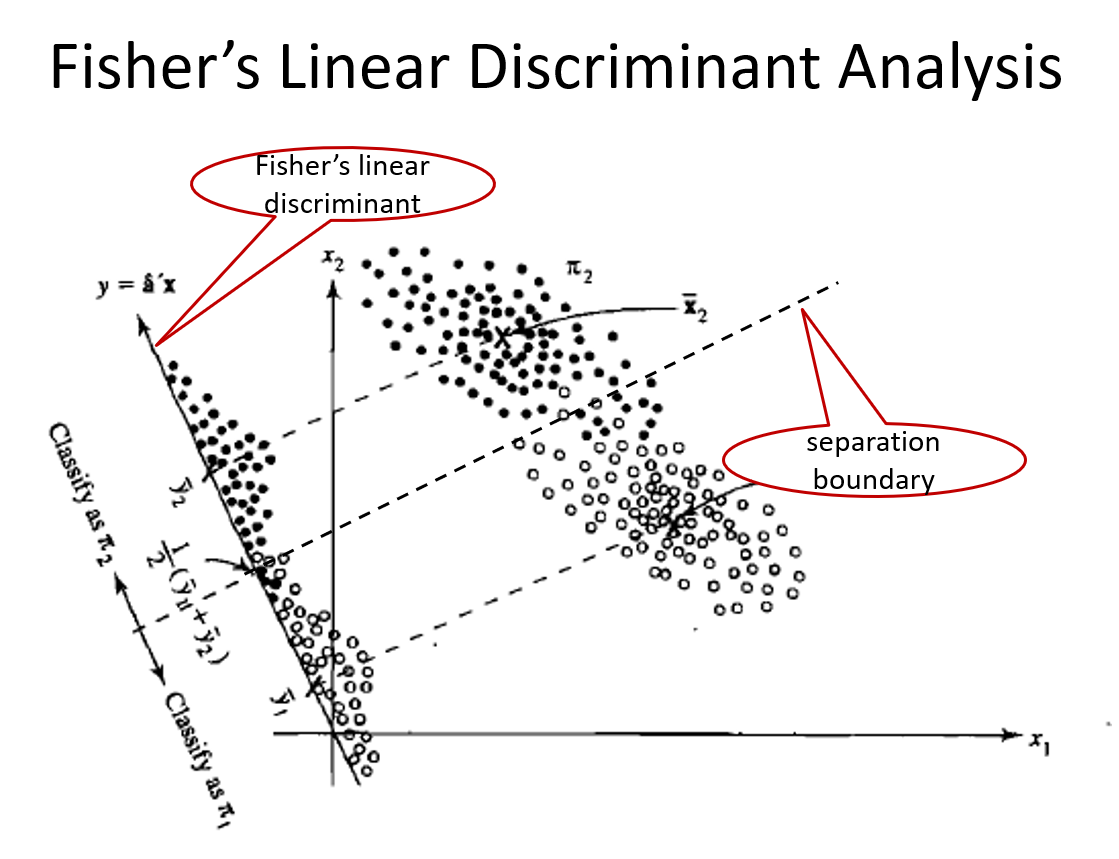
\includegraphics[width=0.7\linewidth]{img/FLDA}
\end{frame}

\hypertarget{two-class-problems}{%
\subsection{Two-Class Problems}\label{two-class-problems}}

\begin{frame}{FLDA: Maximum Separability}
\protect\hypertarget{flda-maximum-separability}{}
\begin{itemize}
\item
  The maximization problem is
  \[\operatorname*{argmax}_a \frac{a^T(\bar {\mathbf X}_1 - \bar {\mathbf X}_2)(\bar {\mathbf X}_1 - \bar {\mathbf X}_2)^Ta}{a^T \boldsymbol \Sigma a}\]
\item
  Use an argument similar to PCA, such \(a\) is the first eigenvector of
  \(\boldsymbol \Sigma ^{-1}(\bar {\mathbf X}_1 - \bar {\mathbf X}_2)(\bar {\mathbf X}_1 - \bar {\mathbf X}_2)^T\).
\item
  We can show that
  \(a=\mathbf S_p^{-1}(\bar {\mathbf X}_1 - \bar {\mathbf X}_2)\).
\item
  The linear function
  \[f(x)=a^T x \mbox{ where } a=\mathbf  S_p^{-1}(\bar {\mathbf X}_1 - \bar {\mathbf X}_2)\]
  is called \textcolor{red}{Fisher's linear discriminant function}.
\end{itemize}
\end{frame}

\begin{frame}{Allocate New Observations}
\protect\hypertarget{allocate-new-observations}{}
\begin{itemize}
\item
  Consider an observation \(X_0\). We compute \[f(X_0)=a^T X_0\] where
  \(a=\mathbf S_p^{-1}(\bar {\mathbf X}_1 - \bar {\mathbf X}_2)\)
\item
  Let
  \[m=a^T \frac{\bar {\mathbf X}_1 + \bar {\mathbf X}_2}{2}=\boldsymbol (\bar {\mathbf X}_1 - \bar {\mathbf X}_2)^T \mathbf  S_p^{-1}\frac{\bar {\mathbf X}_1 + \bar {\mathbf X}_2}{2}\]
\item
  Allocate \(X_0\) to

  \begin{itemize}
  \tightlist
  \item
    class 1 if \(f(X_0)>m\)
  \item
    class 2 if \(f(x_0)<m\)
  \end{itemize}
\end{itemize}
\end{frame}

\hypertarget{g-class-problems}{%
\subsection{g-Class Problems}\label{g-class-problems}}

\begin{frame}{Quantify Separation in a \(g\)-Class Problem}
\protect\hypertarget{quantify-separation-in-a-g-class-problem}{}
\begin{itemize}
\tightlist
\item
  Measure separation using F statistic
\end{itemize}

\[\begin{aligned}
F(a) &= \frac{MSB}{MSW}=\frac{SSB/(g-1)}{SSW/(n-g)}\\
&= \frac{\sum_{i=1}^g n_i (\bar Y_{i.}^{(1)} -\bar Y_{..}^{(1)})^2/(g-1)}{\sum_{i=1}^g (n_i-1)S_{Y_i^{(1)}}^2/(n-g)}\\
&=\frac{a^T \sum n_i (\bar X_{i.} -\bar X_{..})(\bar X_{i.}-\bar X_{..})^T a}{a^T \sum_{i=1}^g\sum_{j=1}^{n_i} (X_{ij} -\bar X_{i.})(X_{ij}-\bar X_{i.})^T a}\frac{n-g}{g-1}\\
&= \frac{a^T \mathbf B a}{a^T \mathbf W a}\frac{n-g}{g-1}
\end{aligned}\] where \(n=\sum_{i=1}^g n_i\), \(\mathbf B\) is the
between-group sample covariance matrix, and \(\mathbf W\) is the
within-group sample covariance matrix.
\end{frame}

\begin{frame}{Linear Discriminants}
\protect\hypertarget{linear-discriminants}{}
\begin{itemize}
\item
  The first linear discriminant is the linear function that maximizes
  \(F(a)\). It can also be shown that the first linear discriminant is
  given by the first eigenvector of \(\mathbf W ^{-1} \mathbf B\), i.e.,
  \[Y_{ij}^{(1)}=\gamma_1^T X_{ij}\] where \(\gamma_1\) is the first
  eigenvector of \(\mathbf W ^{-1} \mathbf B\).
\item
  Similarly, for \(k=1, \cdots, rank(\mathbf B)\), the \(k\)th linear
  discriminant is given by the \(k\)th eigenvector of
  \(\mathbf W ^{-1} \mathbf B\)
\end{itemize}

\[Y_{ij}^{(k)}=\gamma_k^T X_{ij}\]
\end{frame}

\begin{frame}{Use the Linear Discriminants}
\protect\hypertarget{use-the-linear-discriminants}{}
\begin{itemize}
\item
  Let \(X_0\) be a new observation. We allocate it to the group with the
  minimum distance defined by the Euclidean distance in space spanned by
  the linear discriminants.
\item
  Calculate \(Y_0^{(k)}=\gamma_k^T X_0\), the projection of \(X_0\) to
  the \(k\)th linear discriminant for \(k=1, \cdots, rank(B)\).
\item
  Calculate the distance between
  \((Y_0^{(1)}, \cdots, Y_0^{(rank(B))})\) and
  \((\bar Y_{i.}^{(1)}, \cdots, \bar Y_{i.}^{(rank(B))})\)
\end{itemize}

\[D^2(X_0, i) = \sum_{k=1}^{rank(B)} [Y_0^{(k)} - \bar Y_{i.}^{(k)}]^2\]

\begin{itemize}
\tightlist
\item
  Allocate \(X_0\) to \[\operatorname*{argmin}_i D^2(X_0, i)\]
\end{itemize}
\end{frame}

\hypertarget{qda}{%
\section{QDA}\label{qda}}

\hypertarget{qda-for-two-class-problems}{%
\subsection{QDA for Two-Class
Problems}\label{qda-for-two-class-problems}}

\begin{frame}{QDA for Two-Class Problems}
\begin{itemize}
\tightlist
\item
  The LDA can be derived using likelihood functions under the
  assumptions

  \begin{enumerate}
  \tightlist
  \item
    Multivariate normal
  \item
    Equal covariance matrix
  \end{enumerate}
\item
  The assumption of equal covariance matrix is not always a good
  approximation to the true covariance matrices
\item
  If we relax this assumption, we will have QDA
\end{itemize}
\end{frame}

\begin{frame}{QDA for Two-Class Problems}
\protect\hypertarget{qda-for-two-class-problems-1}{}
\begin{itemize}
\item
  Let's consider a two-class classification problem with \(n_1\) and
  \(n_2\) observations in classes 1 and 2, respectively.
\item
  Suppose we have two independent random samples

  \begin{itemize}
  \tightlist
  \item
    Sample 1:
    \(X_{1j}\overset{iid}\sim N(\mathbf \mu_1, \boldsymbol \Sigma_1)\),
    where \(j=1, \cdots, n_1\)
  \item
    Sample 2:
    \(X_{2j}\overset{iid}\sim N(\mathbf \mu_2, \boldsymbol \Sigma_2)\),
    where \(j=1, \cdots, n_2\)
  \end{itemize}
\item
  Sample mean vectors:
  \[\bar {\mathbf X}_1=\frac{1}{n_1}\sum_{j=1}^{n_1}X_{1j}, 
  \bar {\mathbf X}_2=\frac{1}{n_2}\sum_{j=1}^{n_2}X_{2j}\]
\item
  Remark: the sample mean vectors are the MLE of the corresponding mean
  vectors
\end{itemize}
\end{frame}

\begin{frame}{QDA for Two-Class Problems}
\protect\hypertarget{qda-for-two-class-problems-2}{}
\begin{itemize}
\item
  MLE of covariance matrices
  \[\hat {\boldsymbol\Sigma}_1  = \frac{n_1-1}{n_1}S_1, \hat {\boldsymbol\Sigma}_2  = \frac{n_2-1}{n_2}S_2\]
  where \(S_i\) is the sample covariance matrix for sample \(i\).
\item
  Likelihood functions \[\begin{aligned}
  L_1(\boldsymbol \mu_1, \boldsymbol \Sigma_1) \propto |\boldsymbol\Sigma_1|^{-1/2} exp\{-\frac{1}{2} (x-\boldsymbol \mu_1)^T \boldsymbol \Sigma_1^{-1} (x-\boldsymbol \mu_1)\}\\
  L_2(\boldsymbol \mu_2, \boldsymbol \Sigma_2) \propto |\boldsymbol\Sigma_2|^{-1/2} exp\{-\frac{1}{2} (x-\boldsymbol \mu_2)^T \boldsymbol \Sigma_2^{-1} (x-\boldsymbol \mu_2)\}
  \end{aligned}\]
\end{itemize}
\end{frame}

\begin{frame}{QDA for Two-Class Problems}
\protect\hypertarget{qda-for-two-class-problems-3}{}
\begin{itemize}
\tightlist
\item
  We can either check whether the ratio is greater than one or check
  whether the difference of log-likelihood is positive.
\end{itemize}

\[l_1 - l_2=-\frac{1}{2}log(\frac{|\boldsymbol\Sigma_1|}{|\boldsymbol\Sigma_2|}) - \frac{1}{2} [(x-\boldsymbol \mu_1)^T \boldsymbol \Sigma_1^{-1} (x-\boldsymbol \mu_1) - (x-\boldsymbol \mu_2)^T \boldsymbol \Sigma_2^{-1} (x-\boldsymbol \mu_2)]\]

\begin{itemize}
\tightlist
\item
  The classification boundary is given by \(l_1-l_2=0\), i.e.,
\end{itemize}

\[(x-\boldsymbol \mu_1)^T \boldsymbol \Sigma_1^{-1} (x-\boldsymbol \mu_1) - (x-\boldsymbol \mu_2)^T \boldsymbol \Sigma_2^{-1} (x-\boldsymbol \mu_2) = log(\frac{|\boldsymbol\Sigma_2|}{|\boldsymbol\Sigma_1|})\]

\begin{itemize}
\tightlist
\item
  It is quadratic!
\end{itemize}
\end{frame}

\begin{frame}{QDA for Two-Class Problems}
\protect\hypertarget{qda-for-two-class-problems-4}{}
\begin{itemize}
\tightlist
\item
  Replace unknown parameters with estimate, we have the classification
  rule: allocate \(x\) to class 1 if
  \[(x-\bar {\mathbf X}_1)^T \mathbf S _1^{-1} (x-\bar {\mathbf X}_1) - (x-\bar {\mathbf X}_2)^T \mathbf S_2^{-1} (x-\bar {\mathbf X}_2) < log(\frac{|\mathbf S_2|}{|\mathbf S_1|})\]
\end{itemize}
\end{frame}

\begin{frame}{QDA for g-Class Problems}
\protect\hypertarget{qda-for-g-class-problems}{}
\begin{itemize}
\item
  For the \(i\)th group, we compute a quadratic score, which is defined
  as\\
  \[Q_i(x)=(x-\bar {\mathbf X}_i)^T \mathbf S _i^{-1} (x-\bar {\mathbf X}_i)+ log(|\mathbf S_i|)\]
\item
  Allocate \(x\) to the class with the minimum quadratic score
\end{itemize}
\end{frame}

\hypertarget{example-of-qda}{%
\subsection{Example of QDA}\label{example-of-qda}}

\begin{frame}[fragile]{Example of QDA}
\begin{Shaded}
\begin{Highlighting}[]
\NormalTok{obj.lda}\OtherTok{=}\FunctionTok{lda}\NormalTok{(Species}\SpecialCharTok{\textasciitilde{}}\NormalTok{., }\AttributeTok{data =}\NormalTok{ iris)}
\NormalTok{obj.qda}\OtherTok{=}\FunctionTok{qda}\NormalTok{(Species}\SpecialCharTok{\textasciitilde{}}\NormalTok{., }\AttributeTok{data =}\NormalTok{ iris)}

\FunctionTok{table}\NormalTok{(}\AttributeTok{Pred=}\FunctionTok{predict}\NormalTok{(obj.lda, iris)}\SpecialCharTok{$}\NormalTok{class,}
\AttributeTok{True=}\NormalTok{iris}\SpecialCharTok{$}\NormalTok{Species)}
\FunctionTok{table}\NormalTok{(}\AttributeTok{Pred=}\FunctionTok{predict}\NormalTok{(obj.qda, iris)}\SpecialCharTok{$}\NormalTok{class,}
\AttributeTok{True=}\NormalTok{iris}\SpecialCharTok{$}\NormalTok{Species)}
\end{Highlighting}
\end{Shaded}
\end{frame}

\begin{frame}[fragile]{Example of QDA}
\protect\hypertarget{example-of-qda-1}{}
\begin{verbatim}
##             True
## Pred         setosa versicolor virginica
##   setosa         50          0         0
##   versicolor      0         48         1
##   virginica       0          2        49
\end{verbatim}

\begin{verbatim}
##             True
## Pred         setosa versicolor virginica
##   setosa         50          0         0
##   versicolor      0         48         1
##   virginica       0          2        49
\end{verbatim}

\begin{itemize}
\tightlist
\item
  The same result for this particular example
\end{itemize}
\end{frame}

\begin{frame}[fragile]{Visualize QDA Results}
\protect\hypertarget{visualize-qda-results}{}
\begin{Shaded}
\begin{Highlighting}[]
\FunctionTok{partimat}\NormalTok{(Species }\SpecialCharTok{\textasciitilde{}}\NormalTok{ ., }\AttributeTok{data =}\NormalTok{ iris, }\AttributeTok{method =} \StringTok{"qda"}\NormalTok{)}
\end{Highlighting}
\end{Shaded}

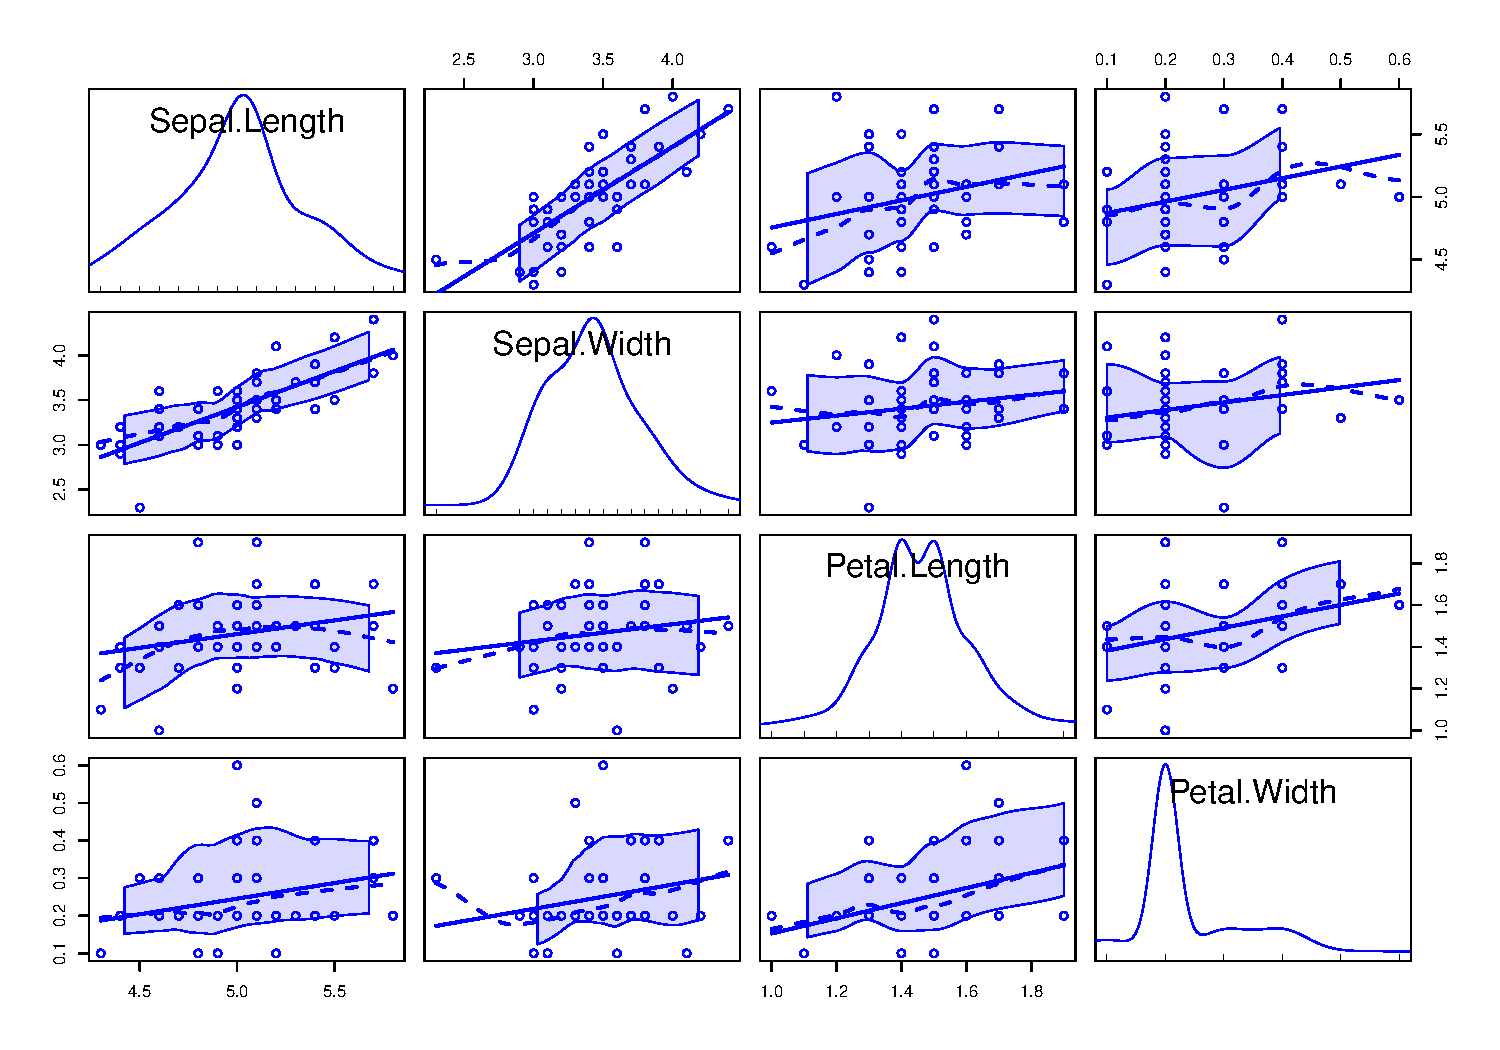
\includegraphics[width=0.8\linewidth]{Lecture14MoreOnClassification_files/figure-beamer/unnamed-chunk-4-1}
\end{frame}

\begin{frame}[fragile]{Visualize LDA Results}
\protect\hypertarget{visualize-lda-results}{}
\begin{Shaded}
\begin{Highlighting}[]
\FunctionTok{partimat}\NormalTok{(Species }\SpecialCharTok{\textasciitilde{}}\NormalTok{ ., }\AttributeTok{data =}\NormalTok{ iris, }\AttributeTok{method =} \StringTok{"lda"}\NormalTok{)}
\end{Highlighting}
\end{Shaded}

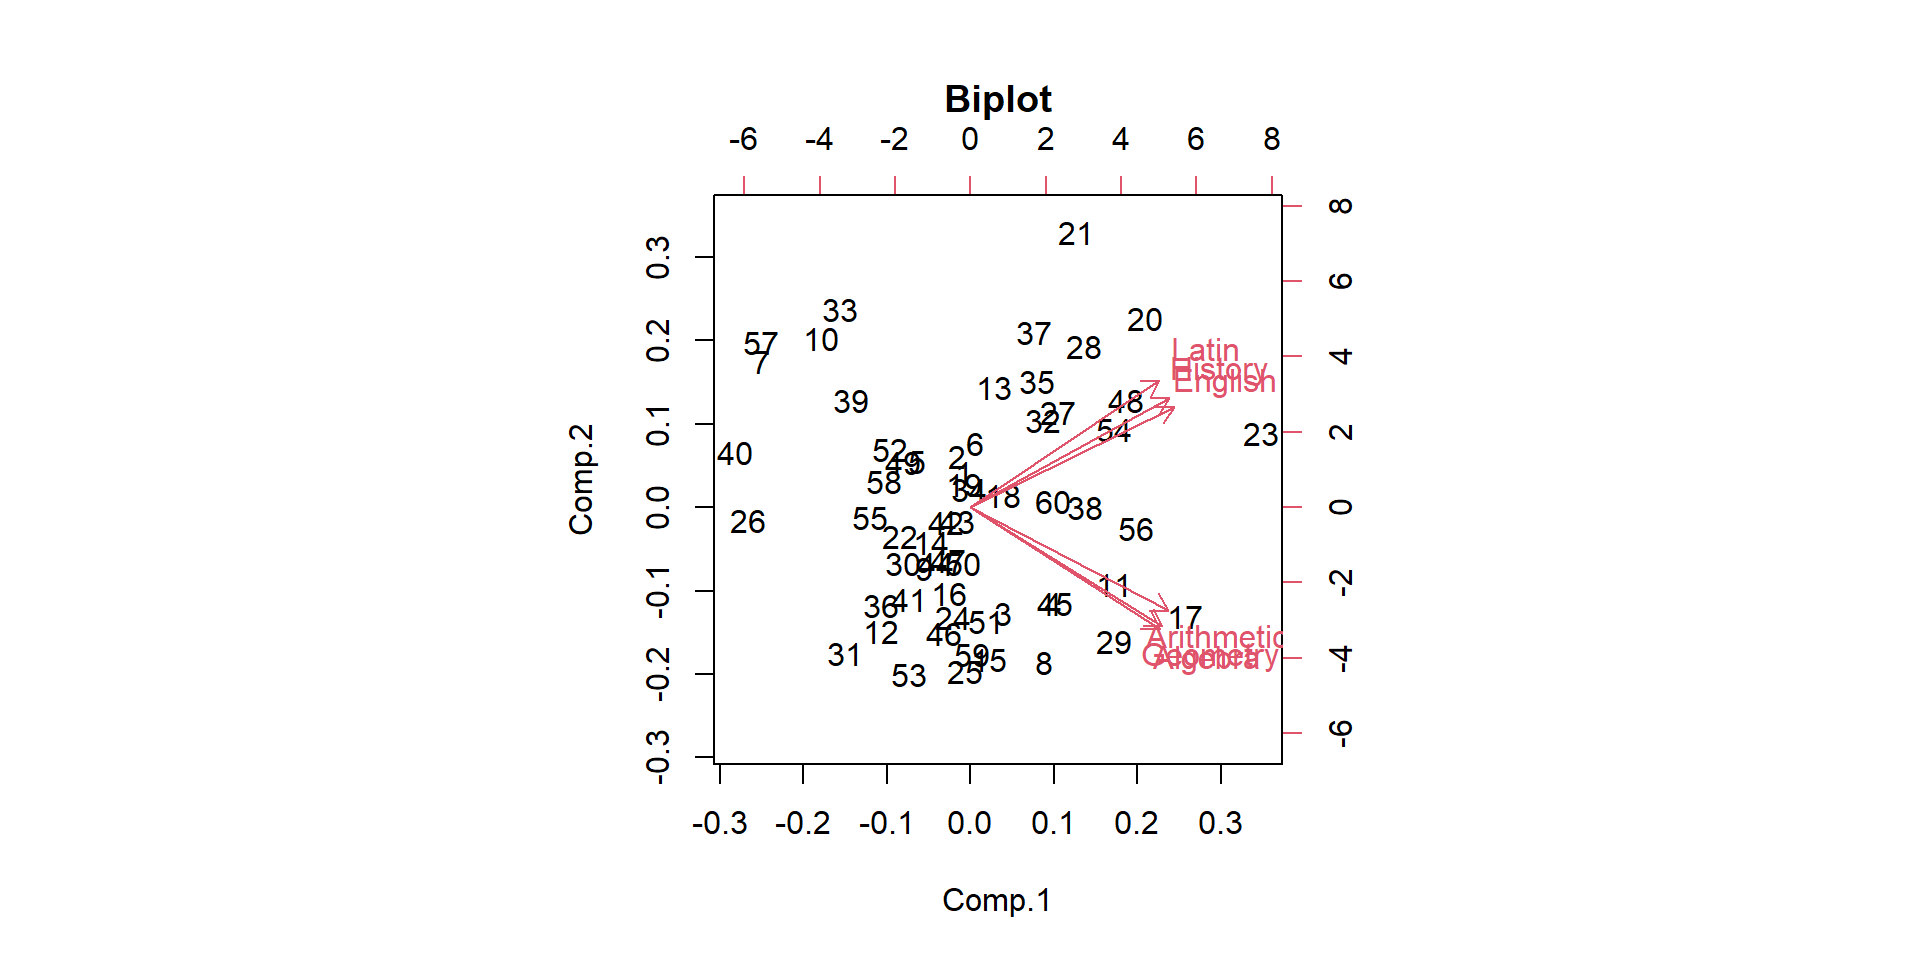
\includegraphics[width=0.8\linewidth]{Lecture14MoreOnClassification_files/figure-beamer/unnamed-chunk-5-1}
\end{frame}

\hypertarget{decision-theory}{%
\section{Decision Theory}\label{decision-theory}}

\begin{frame}{Cost and Prior Probabilities}
\protect\hypertarget{cost-and-prior-probabilities}{}
\begin{itemize}
\tightlist
\item
  In practice, different types of errors have different costs
\item
  Prior probabilities are often known but we haven't discussed how to
  use them
\item
  Goals:

  \begin{itemize}
  \tightlist
  \item
    When different errors have the same cost, we look for a
    classification rule that minimizes the probability of
    misclassification\\
  \item
    When different errors cost differently, we want to find a
    classification rule that minimizes the total cost
  \end{itemize}
\end{itemize}
\end{frame}

\hypertarget{equal-costs}{%
\section{Equal Costs}\label{equal-costs}}

\hypertarget{minimize-probability-of-misclassification}{%
\subsection{Minimize Probability of
Misclassification}\label{minimize-probability-of-misclassification}}

\begin{frame}{Minimize Probability of Misclassification}
\begin{itemize}
\tightlist
\item
  Notations:
\item
  \(X\): data
\item
  \(Z\): true class. It is binary, i.e., \(Z=1\) or \(Z=0\)
\item
  \(P(Z=1)=\pi\): prior probability, known
\item
  \(\delta(x)\): decision function / classifier

  \begin{itemize}
  \tightlist
  \item
    \(\delta(x)=1\): allocate \(x\) to group 1
  \item
    \(\delta(x)=0\): allocate \(x\) to group 0
  \end{itemize}
\end{itemize}
\end{frame}

\begin{frame}{Risk and Posterior Risk}
\protect\hypertarget{risk-and-posterior-risk}{}
\begin{itemize}
\item
  Risk of a classifier \(\delta\) \[\begin{aligned}
  R(\delta, z)&=\Pr [\delta(X)\not= Z|Z=z]=\mathbb E_{X|z} [\mathbb I_{\delta(X)\not= Z}|Z=z]\\
  &=\left\{
  \begin{array}{cc}
  \Pr[\delta(X)=0|z=1] & \mbox{ if } z=1\\
  \Pr[\delta(X)=1|z=0] & \mbox{ if } z=0
  \end{array}\right.
  \end{aligned}\]
\item
  The posterior risk of \(\delta\) \[\begin{aligned}
  PR(\delta(x)) &= \Pr[\delta(x)\not= Z|x]=\mathbb E_{Z|x} [\mathbb I_{\delta(X)\not= Z}|X=x]\\
  &=\left\{
  \begin{array}{cc}
  \Pr[Z=0|x] & \mbox{ if } \delta(x)=1\\
  \Pr[Z=1|x] & \mbox{ if } \delta(x)=0
  \end{array}\right.
  \end{aligned}\]
\end{itemize}
\end{frame}

\begin{frame}{Bayes Risk}
\protect\hypertarget{bayes-risk}{}
\begin{itemize}
\item
  Bayes risk \[B(\delta)=\Pr [\delta(X)\not= Z]\]
\item
  Note that
  \[B(\delta)=\Pr [\delta(X)\not= Z]=\mathbb E_{XZ} [\mathbb I_{\delta(X)\not= Z}]=E_X[PR(\delta, X)]=E_Z[R(\delta, Z)]\]
\item
  Rewrite the Bayes risk \[\begin{aligned}
  B(\delta) &=\Pr [\delta(X)\not= Z]\\
  &=\Pr [\delta(X)=1, Z=0] + \Pr [\delta(X)=0, Z=1]\\
  &=\Pr [\delta(X)=1| Z=0]\Pr[Z=0] + \Pr [\delta(X)=0| Z=1] \Pr[Z=1]\\
  &=\pi \Pr [\delta(X)=0| Z=1]+ (1-\pi)\Pr [\delta(X)=1| Z=0]
  \end{aligned}\]
\item
  The above expression is baesd on the fact
  \[B(\delta)=\mathbb E_{XZ} [\mathbb I_{\delta(X)\not= Z}]\]
\end{itemize}
\end{frame}

\begin{frame}{Bayes Classification Rule}
\protect\hypertarget{bayes-classification-rule}{}
\begin{itemize}
\tightlist
\item
  Want to find \(\delta^*\) that minimizes \(B(\delta)\)
\item
  Claim 1: the \(\delta^*\) that minimizes \(PR(\delta(x))\) also
  minimizes \(B(\delta)\)

  \begin{itemize}
  \tightlist
  \item
    This is because
    \(B(\delta)=\mathbb E[PR(\delta(X)]\ge \mathbb E[PR(\delta^*(X)]=B(\delta^*)\){]}
  \end{itemize}
\item
  Need to find \(\delta^*\) that minimizes \(PR(\delta(x))\). It can be
  shown that
\end{itemize}

\[\delta^*(x)=\left\{
\begin{array}{cc}
1 & \mbox{ if } \frac{\Pr(Z=1|x)}{\Pr(Z=0|x)}>1\\
0 & \mbox{ if } \frac{\Pr(Z=1|x)}{\Pr(Z=0|x)}<1
\end{array}\right.\]

\begin{itemize}
\tightlist
\item
  Skip next slide if you are not interested in the proof
\end{itemize}
\end{frame}

\begin{frame}{The Classifier that Minimizes Posterior Risk}
\protect\hypertarget{the-classifier-that-minimizes-posterior-risk}{}
\begin{itemize}
\tightlist
\item
  Recall that \[PR(\delta(x)=0)=\Pr(Z=1|x), PR(\delta(x)=1)=\Pr(Z=0|x)\]
\item
  Therefore, we \(\delta^*(x)\) should be 1 if \[\begin{aligned}
  PR(\delta(x)=0)>PR(\delta(x)=1) &\Leftrightarrow \Pr(Z=1|x)> \Pr(Z=0|x)\\
  &\Leftrightarrow \frac{\Pr(Z=1|x)}{\Pr(Z=0|x)}>1
  \end{aligned}\]
\end{itemize}
\end{frame}

\begin{frame}{The Bayes Classificatin Rule}
\protect\hypertarget{the-bayes-classificatin-rule}{}
\begin{itemize}
\item
  We say \(\delta^*(x)\) is the Bayes classification rule
  \[\delta^*(x)=\left\{
  \begin{array}{cc}
  1 & \mbox{ if } \frac{\Pr(Z=1|x)}{\Pr(Z=0|x)}>1\\
  0 & \mbox{ if } \frac{\Pr(Z=1|x)}{\Pr(Z=0|x)}<1
  \end{array}\right.\]
\item
  Computation \[\begin{aligned}
  \frac{\Pr(Z=1|x)}{\Pr(Z=0|x)} &
   \overset{\mbox{Bayes' theorem}} = \frac{\frac{f(x|z=1)\Pr(Z=1)}{f(x)}}{\frac{f(x|z=0)\Pr(Z=0)}{f(x)}}\\
  & = \frac{f(x|z=1)}{f(x|z=0)}\frac{\pi}{1-\pi}
  \end{aligned}\]
\item
  A short review of Bayes' theorem is on next slide. Feel free to skip
  if you are very familiar with it already
\end{itemize}
\end{frame}

\begin{frame}{Bayes' Theorem}
\protect\hypertarget{bayes-theorem}{}
\begin{itemize}
\tightlist
\item
  Read this slide if you would like to review Bayes' theorem
\item
  Let \(A\) and \(B\) be two events.
\item
  Bayes' theorem says
  \[\Pr(B|A) = \dfrac{\Pr(A,  B)}{\Pr(A)}=\dfrac{\Pr(A|B)\Pr(B)}{\Pr(A)}\]
  where \(\Pr(A,B)\) means the joint probability that both \(A\) and
  \(B\) occur. We can use alternative expressions such as
  \(\Pr(A \text{ and } B)\) and \(\Pr(A \cap B)\).
\end{itemize}
\end{frame}

\hypertarget{example-1-univariate}{%
\subsection{Example 1: Univariate}\label{example-1-univariate}}

\begin{frame}{Example 1: Univariate}
\begin{itemize}
\tightlist
\item
  Let's consider a univariate example. Suppose that the population
  consists for two underlying populations

  \begin{itemize}
  \tightlist
  \item
    Population 1 with \(\pi\) probability and
    \(N(\mu_1=1, \sigma^2=0.25)\)
  \item
    population 0 with \(1-\pi\) probability and
    \(N(\mu_0=0, \sigma^2=0.25)\)
  \end{itemize}
\item
  Would like to allocate \(x=0.8\)
\item
  According to Bayes classification rule, we need to compute
\end{itemize}

\[\begin{aligned}
\frac{f(x|z=1)\pi}{f(x|z=0)(1-\pi)} &=\frac{f(x|\mu_1=1,\sigma^2)\pi}{f(x|\mu_0=0, \sigma^2)(1-\pi)}\\
&=\frac{\frac{1}{\sigma\sqrt{2\pi}}exp\{-\frac{1}{2\sigma^2}(x-1)^2\}}
{\frac{1}{\sigma\sqrt{2\pi}}exp\{-\frac{1}{2\sigma^2}(x-0)^2\}}\frac{\pi}{1-\pi}\\
&= exp\{\frac{1}{2\sigma^2} (2x-1) \}\frac{\pi}{1-\pi}
\end{aligned}\]
\end{frame}

\begin{frame}{Example 1: Univariate}
\protect\hypertarget{example-1-univariate-1}{}
\begin{itemize}
\item
  The classification boundary is \[\begin{aligned}
  exp\{\frac{1}{2\sigma^2} (2x-1) \} =(1-\pi)/\pi &\Leftrightarrow \frac{1}{2\sigma^2} (2x-1)=log((1-\pi)/\pi)\\
  &\Leftrightarrow x=\sigma^2 log((1-\pi)/\pi)+0.5
  \end{aligned}\]
\item
  The boundary is linear!

  \begin{itemize}
  \tightlist
  \item
    If \(\pi=0.5\), the boundary is \(x=0.5\), we classify \(x=0.8\) to
    class 1.
  \item
    If \(\pi=0.7\), the boundary is \(x=0.288\), we classify \(x=0.8\)
    to class 1.
  \item
    If \(\pi=0.2\), the bondary is \(x=0.846\), we classify \(x=0.8\) to
    class 0.
  \end{itemize}
\end{itemize}
\end{frame}

\begin{frame}{Example 1: Density and Classification Boundary}
\protect\hypertarget{example-1-density-and-classification-boundary}{}
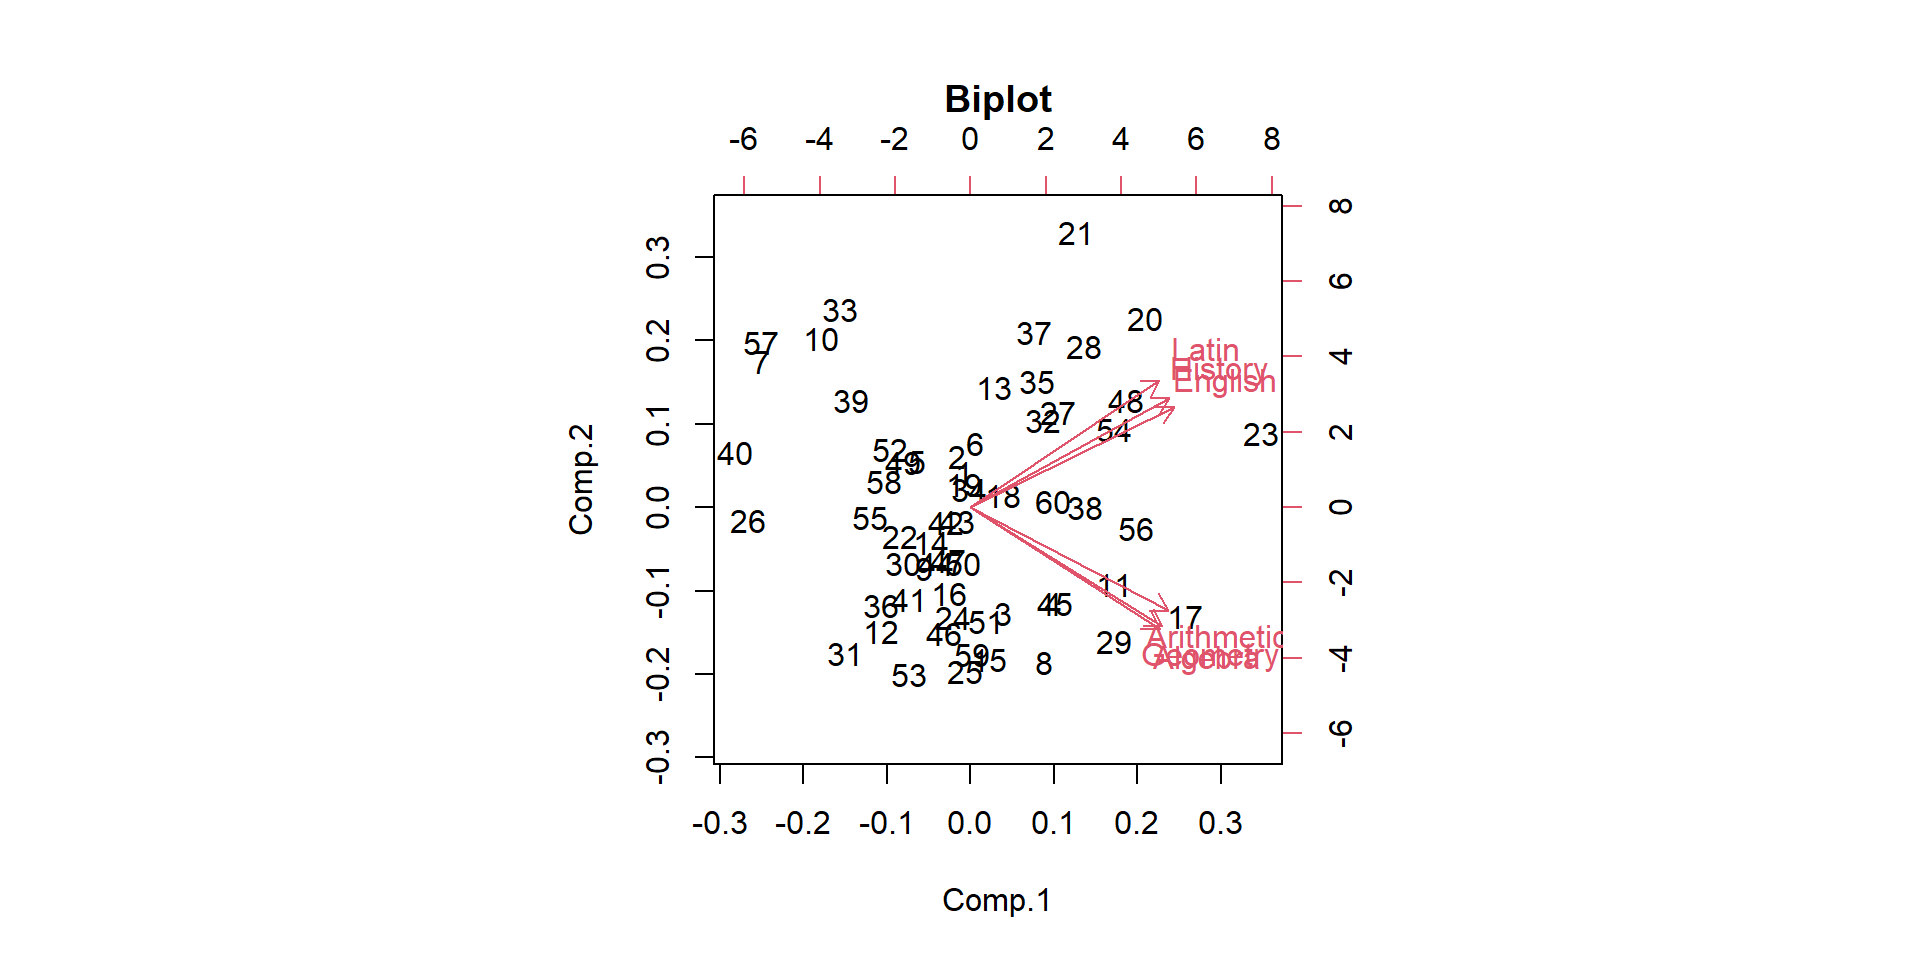
\includegraphics[width=0.8\linewidth]{Lecture14MoreOnClassification_files/figure-beamer/unnamed-chunk-6-1}
\end{frame}

\hypertarget{example-2-multivariate}{%
\subsection{Example 2: Multivariate}\label{example-2-multivariate}}

\begin{frame}{Bayes' Classification under Equal Covariance}
\protect\hypertarget{bayes-classification-under-equal-covariance}{}
\begin{itemize}
\item
  For a two-class problem, the classification boundary by Bayes'
  classification rule is
  \[\frac{f(x|z=1)\pi}{f(x|z=0)(1-\pi)}=1\Leftrightarrow log(\frac{f(x|z=1)}{f(x|z=0)})=log(\frac{1-\pi}{\pi})\]
\item
  Suppose the two underlying distributions are
  \(N(\boldsymbol\mu_1, \boldsymbol \Sigma)\) and
  \(N(\boldsymbol\mu_2, \boldsymbol \Sigma)\).
\item
  The boundary is
  \[-\frac{1}{2}(x-\boldsymbol\mu_1)^T \boldsymbol\Sigma^{-1}(x-\boldsymbol\mu_1) + \frac{1}{2}(x-\boldsymbol\mu_1)^T \boldsymbol\Sigma^{-1}(x-\boldsymbol\mu_1)=log(\frac{1-\pi}{\pi})\]
  which is equivalent to
\end{itemize}

\[(\boldsymbol\mu_1 -\boldsymbol\mu_2)^T \boldsymbol\Sigma^{-1}x = (\boldsymbol\mu_1 -\boldsymbol\mu_2)^T\boldsymbol\Sigma^{-1}\frac{\boldsymbol\mu_1 + \boldsymbol\mu_2}{2} + log(\frac{1-\pi}{\pi})\]
\end{frame}

\begin{frame}{Bayes' Classification under Equal Covariance}
\protect\hypertarget{bayes-classification-under-equal-covariance-1}{}
\begin{itemize}
\item
  In practice, we substitute the unknown parameters by their estimates
  \[(\bar {\mathbf X}_{1.} -\bar {\mathbf X}_{2.})^T\boldsymbol\Sigma^{-1}x = (\bar {\mathbf X}_{1.} -\bar {\mathbf X}_{2.})^T \boldsymbol\Sigma^{-1}\frac{\bar {\mathbf X}_{1.} + \bar {\mathbf X}_{1.}}{2} + log(\frac{1-\pi}{\pi})\]
\item
  Recall that in LDA the linear boundary is
  \[a^Tx=a^T\frac{\bar {\mathbf X}_{1.} + \bar {\mathbf X}_{1.}}{2}\]
  Therefore, Bayes' classification is the same as the LDA when
  \(\pi=1/2\).
\item
  Similarly, in a g-class problem, LDA is the same as Bayes
  classification under the assumptions (1) multivariate normality, (2)
  equal covariance, and (3) uniform prior probabilities.
\end{itemize}
\end{frame}

\begin{frame}{Connection with Logistic Regression}
\protect\hypertarget{connection-with-logistic-regression}{}
\begin{itemize}
\tightlist
\item
  A logistic regression can be used for a two-class problem
\item
  It models the log-odds, which is defined as
  \[\frac{\Pr(Z=1|x)}{{\Pr(Z=0|x)}}\] This is the ratio of posterior
  risks.
\item
  More specifically, it models the log-odds as a linear function of the
  covariates.
\item
  The LDA under the Bayes rule computes the ratio of the posterior risk.
  The decision function is also based on a linear function of the
  covariates.
\item
  Therefore we see a connection between them.
\item
  The two approaches were derived from different models with different
  assumptions.

  \begin{itemize}
  \tightlist
  \item
    Logistic regression models \ldots{}
  \item
    LDA models \ldots{}
  \end{itemize}
\end{itemize}
\end{frame}

\hypertarget{example-3-univariate-unequal-variance}{%
\subsection{Example 3: Univariate, Unequal
Variance}\label{example-3-univariate-unequal-variance}}

\begin{frame}{Example 3: Univariate, Unequal Variance}
\begin{itemize}
\tightlist
\item
  Again, consider a univariate example. This time we relax the
  assumption of equal variance
\item
  Suppose that the population consists for two underlying populations

  \begin{itemize}
  \tightlist
  \item
    Population 1 with \(\pi\) probability and
    \(N(\mu_1=1, \sigma_1^2=0.25)\)
  \item
    population 0 with \(1-\pi\) probability and
    \(N(\mu_0=0, \sigma_2^2=1)\)
  \end{itemize}
\item
  Would like to allocate \(x=0.8\)
\end{itemize}
\end{frame}

\begin{frame}{Example 3: Univariate, Unequal Variance}
\protect\hypertarget{example-3-univariate-unequal-variance-1}{}
\begin{itemize}
\item
  According to Bayes classification rule, we need to compute
  \[\begin{aligned}
  \frac{f(x|z=1)\pi}{f(x|z=0)(1-\pi)} &=\frac{f(x|\mu_1=1,\sigma_1^2)\pi}{f(x|\mu_0=0, \sigma_0^2)(1-\pi)}\\
  &=\frac{\frac{1}{\sigma_1\sqrt{2\pi}}exp\{-\frac{1}{2\sigma_1^2}(x-1)^2\}}
  {\frac{1}{\sigma_0\sqrt{2\pi}}exp\{-\frac{1}{2\sigma_0^2}(x-0)^2\}}\frac{\pi}{1-\pi}\\
  &= exp\{(\frac{1}{2\sigma_0^2}-\frac{1}{2\sigma_1^2})x^2 + \frac{x}{\sigma_1^2}-\frac{1}{2\sigma_1^2}\}
  \frac{\pi}{1-\pi}\frac{\sigma_0}{\sigma_1}
  \end{aligned}\]
\item
  The classification boundary is
  \[(\frac{1}{2\sigma_0^2}-\frac{1}{2\sigma_1^2})x^2 + \frac{x}{\sigma_1^2}-\frac{1}{2\sigma_1^2}=log[
  \frac{1-\pi}{\pi}\frac{\sigma_1}{\sigma_0}]
  \]
\item
  It is quadratic!
\end{itemize}
\end{frame}

\begin{frame}[fragile]{Example 3: Univariate, Unequal Variance}
\protect\hypertarget{example-3-univariate-unequal-variance-2}{}
\tiny

\begin{Shaded}
\begin{Highlighting}[]
\NormalTok{mean1 }\OtherTok{\textless{}{-}} \DecValTok{1}
\NormalTok{var1 }\OtherTok{\textless{}{-}} \FloatTok{0.25}
\NormalTok{mean0 }\OtherTok{\textless{}{-}} \DecValTok{0}
\NormalTok{var0 }\OtherTok{\textless{}{-}} \FloatTok{0.64}
\NormalTok{weight1 }\OtherTok{\textless{}{-}} \FloatTok{0.5}
\NormalTok{weight0 }\OtherTok{\textless{}{-}} \DecValTok{1} \SpecialCharTok{{-}}\NormalTok{ weight1}

\CommentTok{\# doesn\textquotesingle{}t seem to be correct}
\NormalTok{x }\OtherTok{\textless{}{-}} \FunctionTok{seq}\NormalTok{(}\SpecialCharTok{{-}}\DecValTok{2}\NormalTok{, }\DecValTok{3}\NormalTok{, }\AttributeTok{length.out =} \DecValTok{1000}\NormalTok{)}
\NormalTok{fx}\OtherTok{=}\NormalTok{(}\DecValTok{1}\SpecialCharTok{/}\NormalTok{var0 }\SpecialCharTok{{-}} \DecValTok{1}\SpecialCharTok{/}\NormalTok{var1)}\SpecialCharTok{/}\DecValTok{2}\SpecialCharTok{*}\NormalTok{x}\SpecialCharTok{\^{}}\DecValTok{2} \SpecialCharTok{+}\NormalTok{ x}\SpecialCharTok{/}\NormalTok{var1 }\SpecialCharTok{{-}} \DecValTok{1}\SpecialCharTok{/}\DecValTok{2}\SpecialCharTok{/}\NormalTok{var1 }\SpecialCharTok{{-}} \FunctionTok{log}\NormalTok{(weight0}\SpecialCharTok{*}\FunctionTok{sqrt}\NormalTok{(var1)}\SpecialCharTok{/}\NormalTok{weight1}\SpecialCharTok{/}\FunctionTok{sqrt}\NormalTok{(var0))}
\FunctionTok{plot}\NormalTok{(x, fx, }\AttributeTok{type=}\StringTok{"n"}\NormalTok{)}
\FunctionTok{lines}\NormalTok{(x[fx}\SpecialCharTok{\textgreater{}}\DecValTok{0}\NormalTok{], fx[fx}\SpecialCharTok{\textgreater{}}\DecValTok{0}\NormalTok{], }\AttributeTok{col=}\StringTok{"blue"}\NormalTok{)}
\FunctionTok{lines}\NormalTok{(x[fx}\SpecialCharTok{\textless{}}\DecValTok{0}\NormalTok{], fx[fx}\SpecialCharTok{\textless{}}\DecValTok{0}\NormalTok{], }\AttributeTok{col=}\StringTok{"green"}\NormalTok{)}
\FunctionTok{abline}\NormalTok{(}\AttributeTok{h=}\DecValTok{0}\NormalTok{)}
\end{Highlighting}
\end{Shaded}

\normalsize
\end{frame}

\begin{frame}{Example 3: Univariate, Unequal Variance}
\protect\hypertarget{example-3-univariate-unequal-variance-3}{}
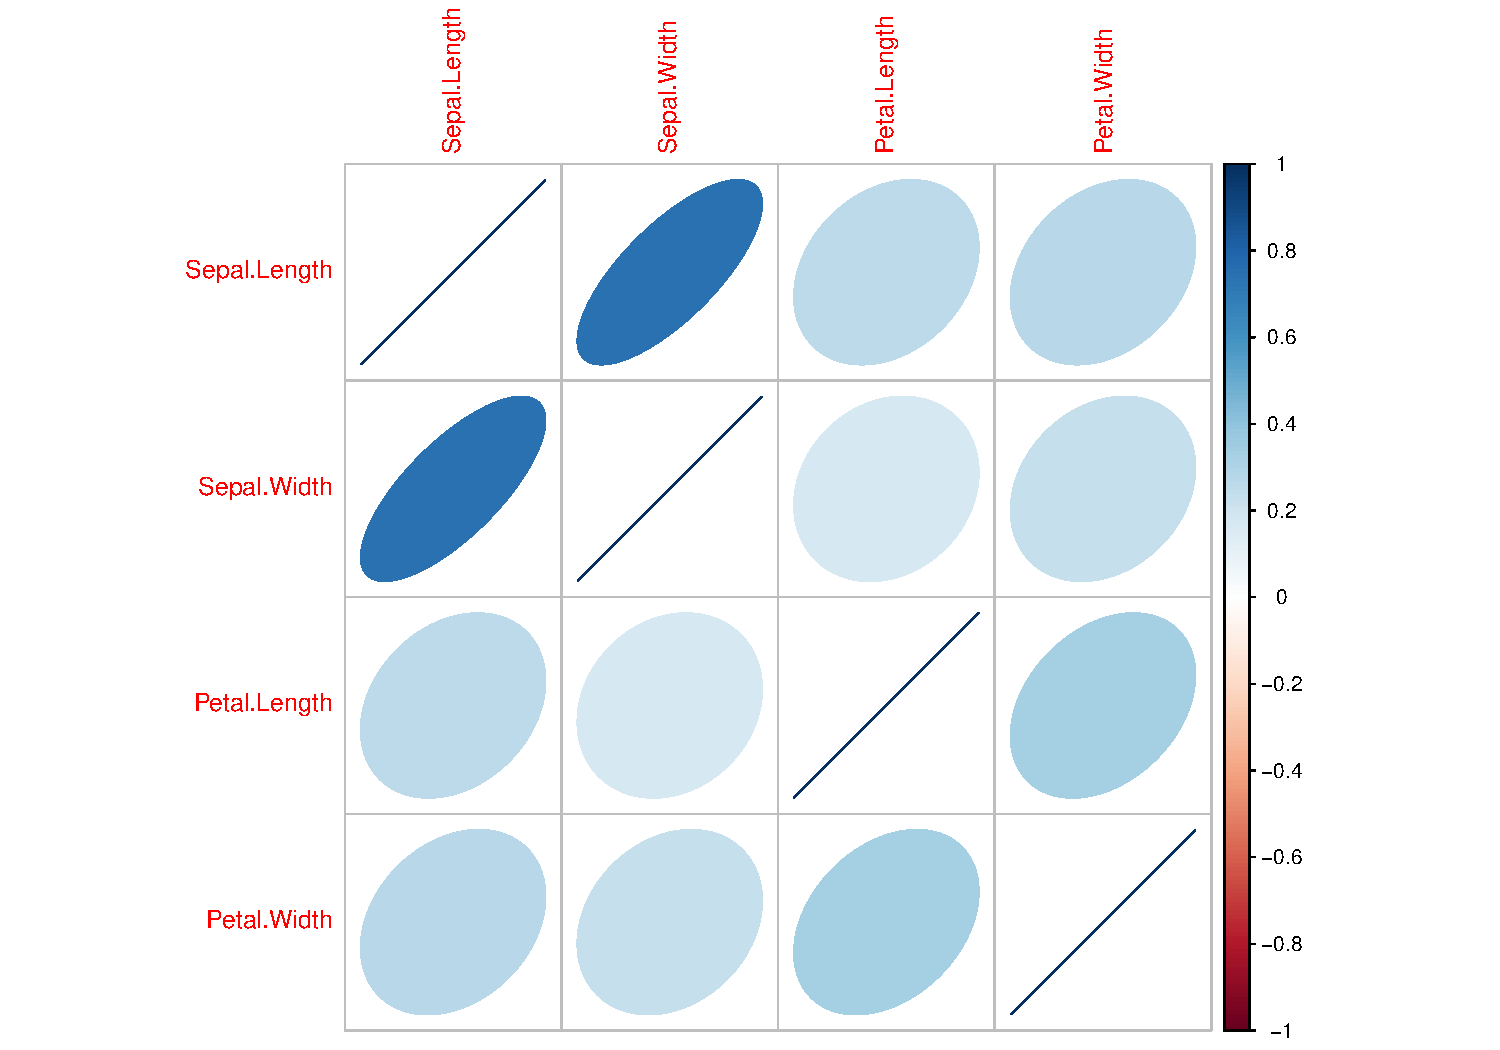
\includegraphics[width=0.8\linewidth]{Lecture14MoreOnClassification_files/figure-beamer/unnamed-chunk-8-1}
\end{frame}

\hypertarget{unequal-costs}{%
\section{Unequal Costs}\label{unequal-costs}}

\hypertarget{risk-and-cost}{%
\subsection{Risk and Cost}\label{risk-and-cost}}

\begin{frame}{Risk and Cost}
\begin{itemize}
\tightlist
\item
  Different types of misclassifications might cost differently
\item
  Let \(L(\delta(x), z)\) denote the cost function
\item
  Let \(C(1|0)=L(1, 0)\), the cost of misclassifying 0 to 1
\item
  Let \(C(0|1)=L(0, 1)\), the cost of misclassifying 1 to 0
\item
  The Risk and Bayes risk need to be revised accordingly
\end{itemize}
\end{frame}

\begin{frame}{Risk and Posterior Risk}
\protect\hypertarget{risk-and-posterior-risk-1}{}
\begin{itemize}
\item
  Risk of a classifier \(\delta\)
  \[R(\delta, z)=\mathbb E_{X|Z=z} [L(\delta(X), z)]=\left\{
  \begin{array}{cc}
  C(0|1)\Pr[\delta(X)=0|z=1] & \mbox{ if } z=1\\
  C(1|0)\Pr[\delta(X)=1|z=0] & \mbox{ if } z=0
  \end{array}\right.\]
\item
  The posterior risk of \(\delta\) \[\begin{aligned}
  PR(\delta(x)) &= \mathbb E_{Z|x}[L(\delta(x), Z)]\\
  &=\left\{
  \begin{array}{cc}
  C(1|0)\Pr[Z=0|x] & \mbox{ if } \delta(x)=1\\
  C(0|1)\Pr[Z=1|x] & \mbox{ if } \delta(x)=0
  \end{array}\right.
  \end{aligned}\]
\end{itemize}
\end{frame}

\begin{frame}{Bayes Risk}
\protect\hypertarget{bayes-risk-1}{}
\begin{itemize}
\tightlist
\item
  Bayes risk \[B(\delta)=\mathbb E_{XZ} [L(\delta(X), Z)]\]
\item
  Rewrite the Bayes risk
\end{itemize}

\tiny

\[\begin{aligned}
B(\delta) &=\mathbb E_{XZ} [L(\delta(X), Z)]\\
&=L(\delta(X)=1, Z=0)\Pr[\delta(X)=1, Z=0] + L(\delta(X)=0, Z=1)[\delta(X)=0, Z=1]\\
&=C(1|0)\Pr [\delta(X)=1, Z=0] + C(0|1)\Pr [\delta(X)=0, Z=1]\\
&=C(1|0)\Pr [\delta(X)=1| Z=0]\Pr[Z=0] + C(0|1)\Pr [\delta(X)=0| Z=1] \Pr[Z=1]\\
&=C(0|1)\pi \Pr [\delta(X)=0| Z=1]+ (1-\pi)C(1|0)\Pr [\delta(X)=1| Z=0]
\end{aligned}\] \normalsize
\end{frame}

\begin{frame}{Bayes Classification Rule with Unequal Costs}
\protect\hypertarget{bayes-classification-rule-with-unequal-costs}{}
\begin{itemize}
\tightlist
\item
  Use a derivation similar to the equal cost situation, we can show that
  the Bayes classification rule is
\end{itemize}

\[\begin{aligned}
&PR(\delta(x)=0)>PR(\delta(x)=1) \\
&\Leftrightarrow C(0|1)\Pr(Z=1|x)> C(1|0)\Pr(Z=0|x)\\
&\Leftrightarrow \frac{\Pr(Z=1|x)}{\Pr(Z=0|x)}>\frac{C(1|0)}{C(0|1)}\\
&\Leftrightarrow \frac{f(x|z=1)}{f(x|z=0)}>\frac{C(1|0)}{C(0|1)}\frac{1-\pi}{\pi}
\end{aligned}\]
\end{frame}

\begin{frame}{Other Related Topics}
\protect\hypertarget{other-related-topics}{}
\begin{itemize}
\tightlist
\item
  There are numerous issues/methods / models
\item
  Training error vs testing error
\item
  Model / variable selection / shrinkage
\item
  Classification tree. Random forest
\item
  Support vector machine
\item
  Neural network and deep neural network
\end{itemize}
\end{frame}

\end{document}
